
% Chapter 2
\Chapter{MSSCopilot}{Generación de Código Automática}

\section{Objetivo de las prácticas}
El objetivo principal de las prácticas fue desarrollar una herramienta que permitiera a los usuarios generar código de manera automática. Esta herramienta, denominada MSSCopilot, debía ser capaz de generar código en \href{https://dotnet.microsoft.com/es-es/languages/csharp}{\bold{C\#}} / \href{https://en.wikipedia.org/wiki/Language_Integrated_Query}{\bold{LINQ}} a partir de la base de código fuente existente en la compañía.

\begin{examplebox}

Un empleado le dice al MSSCopilot que desea obtener una lista con todos los Warehouses, el Copilot respondería con un código como el siguiente:

\begin{lstlisting}[language=C]
    using (var context = new MyContext())
    {
        var result = context.Warehouse.Select(x => x);
    }
    \end{lstlisting}
\end{examplebox}        

Durante el desarrollo del programa se elaboraron más funcionalidades de las previstas inicialmente como es la explicación de código, y otras más que se explicarán con mayor profundidad posteriormente.

El estado del proyecto al comenzar las prácticas estaba en una etapa inicial, lo que permitió un entendimiento más profundo del mismo y facilitó la integración de nuevas ideas y funcionalidades desde el principio. 

\section{Desarrollo}

Definir las tecnologías utilizadas en la realización del MSSCopilot resulta complicado porque como se ha comentado en la sección \ref{sec:contexto}, aunque se trate de desarrollar un producto de software, ha sido un proyecto en el que, por la naturaleza de la IA, que sigue siendo un sector de tecnologías emergentes, las directrices a seguir no son tan claras. Debido a esto, gran parte del proyecto ha consistido en un proceso de investigación en el que se han utilizado tecnologías y técnicas que, con el tiempo, se han descartado en favor de otras opciones mejores a medida que se identificaban. Hay mucho trabajo realizado que he omitido porque la memoria de prácticas no pretende ser una memoria técnica, sin embargo, es importante tener en cuenta que estas tecnologías y explicaciones son solo una parte del panorama completo, y el proyecto ha implicado una exploración más amplia de diversas herramientas y enfoques en el campo de la inteligencia artificial.

\subsection{Conocimientos previos}
Los \href{https://en.wikipedia.org/wiki/Large_language_model}{\bold{LLM}} son un tipo de modelo de inteligencia artificial diseñado para comprender y generar texto, como es el famoso \href{https://es.wikipedia.org/wiki/GPT-4}{\bold{GPT}}, para este proyecto se ha utilizado \href{https://ollama.com/}{\bold{Ollama}}.

En la descripción de las prácticas una de las tareas fundamentales era diseñar y entrenar el sistema a partir de la base de código fuente existente en la
compañía. Para entrenar un \href{https://en.wikipedia.org/wiki/Large_language_model}{\bold{LLM}} con información nueva hay dos opciones:
\begin{itemize}
    \item Ajustar el modelo preentrenado utilizando un cojunto de datos más pequeño y específico, proceso conocido como \bold{Fine-tuning.}
    \item Convertir palabras, frases o textos completos en vectores numéricos. Estos \bold{Embeddings} capturan el significado y las relaciones semánticas del texto. Se pueden convertir las preguntas del usuario en embeddings y compararlos con los embeddings de la información que tenemos almacenada en una BDD, y si ambos tienen x similitud darle esa información al \href{https://en.wikipedia.org/wiki/Large_language_model}{\bold{LLM}} en tiempo real para que responda con nuestra información.
\end{itemize}



En resumen, en la primera opción ponemos al modelo a estudiar los conocimientos nuevos generando así un nuevo modelo, y en la segunda opción es como si el modelo para cada pregunta, consultase en un diccionario/libro con respuestas, buscando la que más se parezca a la pregunta del usuario.  

Durante el transcurso de las prácticas he tenido que realizar el programa utilizando ambas opciones.

\newpage
\subsection{Embeddings}
Inicialmente se optó por utilizar Embeddings, usando \href{https://www.sqlite.org/}{\bold{SQLite}} para la BDD, y \href{https://dotnet.microsoft.com/es-es/languages/csharp}{\bold{C\#}} por compatibilidad con toda la infraestructura de la empresa, permitiendo el poder integrar a futuro esta utilidad de asistente de código a todos los servicios que ofrecen.

La base de datos contenía queries correctamente escritas en \href{https://dotnet.microsoft.com/es-es/languages/csharp}{\bold{C\#}} junto con su respectiva descripción, y el embedding asociado, esto se descartó posteriormente ya que no era viable para la empresa ponerse a generar queries con descripciones para cada casuística, y en versiones posteriores se optaría por pasarle el contenido de las tablas. Para generar la BDD se creó una clase que lee archivos de código fuente \href{https://dotnet.microsoft.com/es-es/languages/csharp}{\bold{C\#}} de la empresa que se filtran para extraer el contenido. Con las tablas el procedimiento fue el mismo, gracias al uso de \href{https://en.wikipedia.org/wiki/Entity_Framework}{\bold{Entity Framework}}. 

\newpage
Dicha comparación que se realiza entre Embeddings de la pregunta del usuario y la BDD se tuvo que implementar en código, se implementó tanto la similitud coseno como la euclídea:


\begin{figure}[htbp]
    \centering
    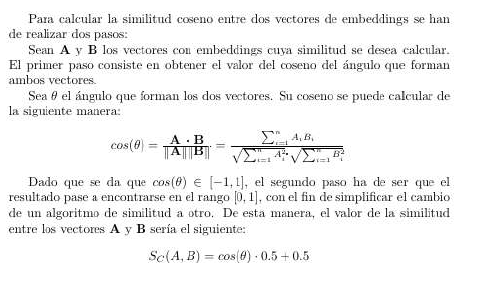
\includegraphics[width=0.8\textwidth]{Chapters/cap4.PNG}
    \label{fig:mi_imagen}
\end{figure}

\begin{figure}[htbp]
    \centering
    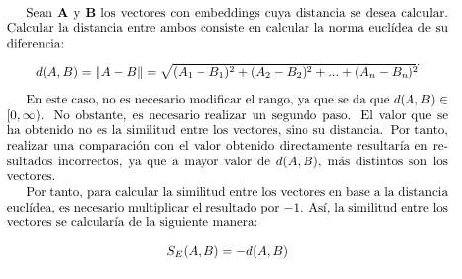
\includegraphics[width=0.8\textwidth]{Chapters/cap5.PNG}
    \label{fig:mi_imagen2}
\end{figure}

Se optó por utilizar la distancia euclídea.

\newpage

Con estas tecnologías y métodos se creó la primera versión funcional del Copilot, de la que sugieron múltiples versiones y mejoras que se aplicaron en cada una de ellas.

Algunas de las mejoras que se fueron aplicando tras prueba y error:

\begin{itemize}
    \item Se realizaron pruebas con diferentes modelos de \href{https://ollama.com/}{\bold{Ollama}} y se optó por el codellama-instruct, por su capacidad para generar código correctamente y también explicarlo. Nos dimos cuenta que aún codellama siendo un modelo especializado en código, su variante Instruct le confería la capacidad de explicar código y por ende tenía un procesamiento del lenguaje natural superior que otras versiones de codellama no disponía. Probamos convirtiendo las tablas de la BDD al lenguaje natural y tanto la comprensión del modelo como la similitud de los embeddings mejoró sustancialmente.
    \begin{figure}[htbp]
        \centering
        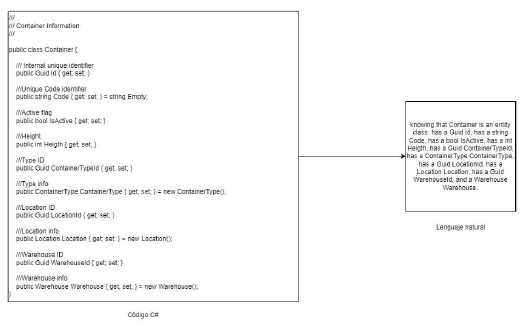
\includegraphics[width=0.9\textwidth]{Chapters/cap6.PNG}
        \label{fig:mi_imagen3}
    \end{figure}
    \item Se optó por dejar de lado \href{https://www.sqlite.org/}{\bold{SQLite}} para utilizar \href{https://www.postgresql.org/}{\bold{PostgreSQL}} junto con un módulo lllamado pgvector especializado en operaciones vectoriales que ya contaba con operaciones de distancia euclídea, por lo que no había necesidad de seguir usando código propio en \href{https://dotnet.microsoft.com/es-es/languages/csharp}{\bold{C\#}}, lo cual disminuyó enormemente los tiempos de respuesta.
    \item Se hicieron benchmarks y comparaciones entre el modo normal de funcionamiento del modelo en el que guarda el historial de todo lo que se ha escrito para poder responder a preguntas anteriores, y el modo stateless en el que no guarda información entre preguntas.
    \item Se implementó un mecanismo para detectar que la pregunta del usuario está pidiendo una explicación, preparando al modelo para que responda correctamente.
    \item Se diseñaron métodos para mejorar el tiempo de respuesta del Copilot, ya que se pretendía utilizar el hardware de los equipos de los trabajadores, por lo que tenía que ser capaz de responder en un tiempo aceptable incluso con hardware modesto.
    \item Se creó un menú inicial a la hora de arrancar el programa(se ejecuta en una terminal), en el que te permite escoger el modelo \href{https://en.wikipedia.org/wiki/Large_language_model}{\bold{LLM}} que se desee, y un submenú con todas las diferentes configuraciones creadas y tecnologías utilizadas a lo largo de las prácticas, como puede ser utilizar el Copilot en modo stateless o no, usar \href{https://www.postgresql.org/}{\bold{PostgreSQL}} o \href{https://www.sqlite.org/}{\bold{SQLite}}, o utilizar Embeddings o no. 
\end{itemize}

\subsection{Fine-tuning}

Una vez que la versión con Embeddings era funcional, y respondía en unos tiempos aceptables, se optó por probar el Fine-tuning para comparar los tiempos de respuesta.

Esta decisión era algo que personalmente desde el principio descartaba porque requiere un gasto computacional enorme y se requieren de muchísimos datos para que el Fine-tuning pueda tener un impacto significativo en el modelo, cosa en la que el tutor de prácticas estuvo de acuerdo por lo que esta etapa estaba inicialmente destinada a estimar cuanto podría llegar a costar hacerlo, y como hacerlo.

Investigando sobre el Fine-tuning descubrí un método llamado LoRA para poder hacer Fine-tuning sin tener que preentrenar el modelo \href{https://en.wikipedia.org/wiki/Large_language_model}{\bold{LLM}} entero, facilita la adaptación de modelos de lenguaje preentrenados a nuevas tareas sin un reinicio completo del entrenamiento, digamos que es como acoplar al modelo preexistente, en este caso Codellama, otro 'modelo' LoRA en tiempo de ejecución.

Esto viene muy bien a \href{https://www.mecalux.es/}{\bold{Mecalux}} no solo porque se ahorraría los costes de un Fine-tuning clásico, sino que si su base de datos crece, no es necesario volver a entrenar de cero el modelo, varios adaptadores LoRA pueden ser aplicados a un mismo modelo, y la generación de estos adaptadores es muy poco costosa computacionalmente.

Para esta nueva etapa el código en \href{https://dotnet.microsoft.com/es-es/languages/csharp}{\bold{C\#}} no cambió demasiado, y el tiempo fue destinado en como generar estos adaptadores. Llamasharp que es la biblioteca \href{https://dotnet.microsoft.com/es-es/languages/csharp}{\bold{C\#}}/.NET usada para ejecutar \href{https://en.wikipedia.org/wiki/Large_language_model}{\bold{LLM}} era incapaz de utilizar estos adaptadores correctamente, por lo que sabiendo que está basado en el proyecto original de \href{https://ollama.com/}{\bold{Ollama}} llama.cpp, escrito en \href{https://en.wikipedia.org/wiki/C_(programming_language)}{\bold{C}}/\href{https://en.wikipedia.org/wiki/C%2B%2B}{\bold{C++}} y \href{https://www.python.org/}{\bold{Python}}, se probó a utilizar los adaptadores generados en \href{https://en.wikipedia.org/wiki/C%2B%2B}{\bold{C++}} desde un Ubuntu, y se confirmó que allí si funcionaba. Aunque nos encontramos con ese bug el cual fue notificado, tuvimos la suerte de poder utilizar uno de los programas en \href{https://www.python.org/}{\bold{Python}} que vienen dentro del proyecto de llama.cpp que permite fusionar el modelo base con el adaptador LoRA y generar un modelo nuevo, que a efectos prácticos es lo mismo.

Como el proceso de generar adaptadores y combinarlos era una tarea muy tediosa y que requería de cierta complejidad y conocimientos realicé un programa en shell script para facilitar todo el proceso y de paso generar métricas. Por ejemplo la cantidad requerida de RAM para generar los adaptadores era muy elevada y sobrepasaba con creces la de los portátiles de trabajo de la empresa, por tanto el script se encarga de generar memoria swap en este caso, evitando un fallo de segmentación.

\subsection{Embeddings vs Fine-tuning}
Al finalizar las prácticas se hicieron los benchmarks pertinentes y en cuanto a tiempos de ejecución ambos eran similares, en parte porque se dedicó mucho esfuerzo en optimizar al máximo la opción embeddings, pero en la resolución de las preguntas y en coherencia tanto en las explicaciones como en la generación de código ganaba los Embeddings.

La explicación a esto además de lo previamente mencionado es que el adaptador necesita de un fichero con la información que se quiere aprender, y no había mucha información en cuanto a como de redactar dicho fichero, se probó a escribirlo en lenguaje natural y después siguiendo directrices que se usaron para entrenar a codellama, pero no se hicieron unas pruebas exhaustivas por no disponer de más tiempo.

Es probable que afinando la manera de elaborar ese fichero las comparativas cambien a favor del Fine-tuning usando LoRA.
\subsection{Esquema general del proyecto}

\begin{figure}[htbp]
    \centering
    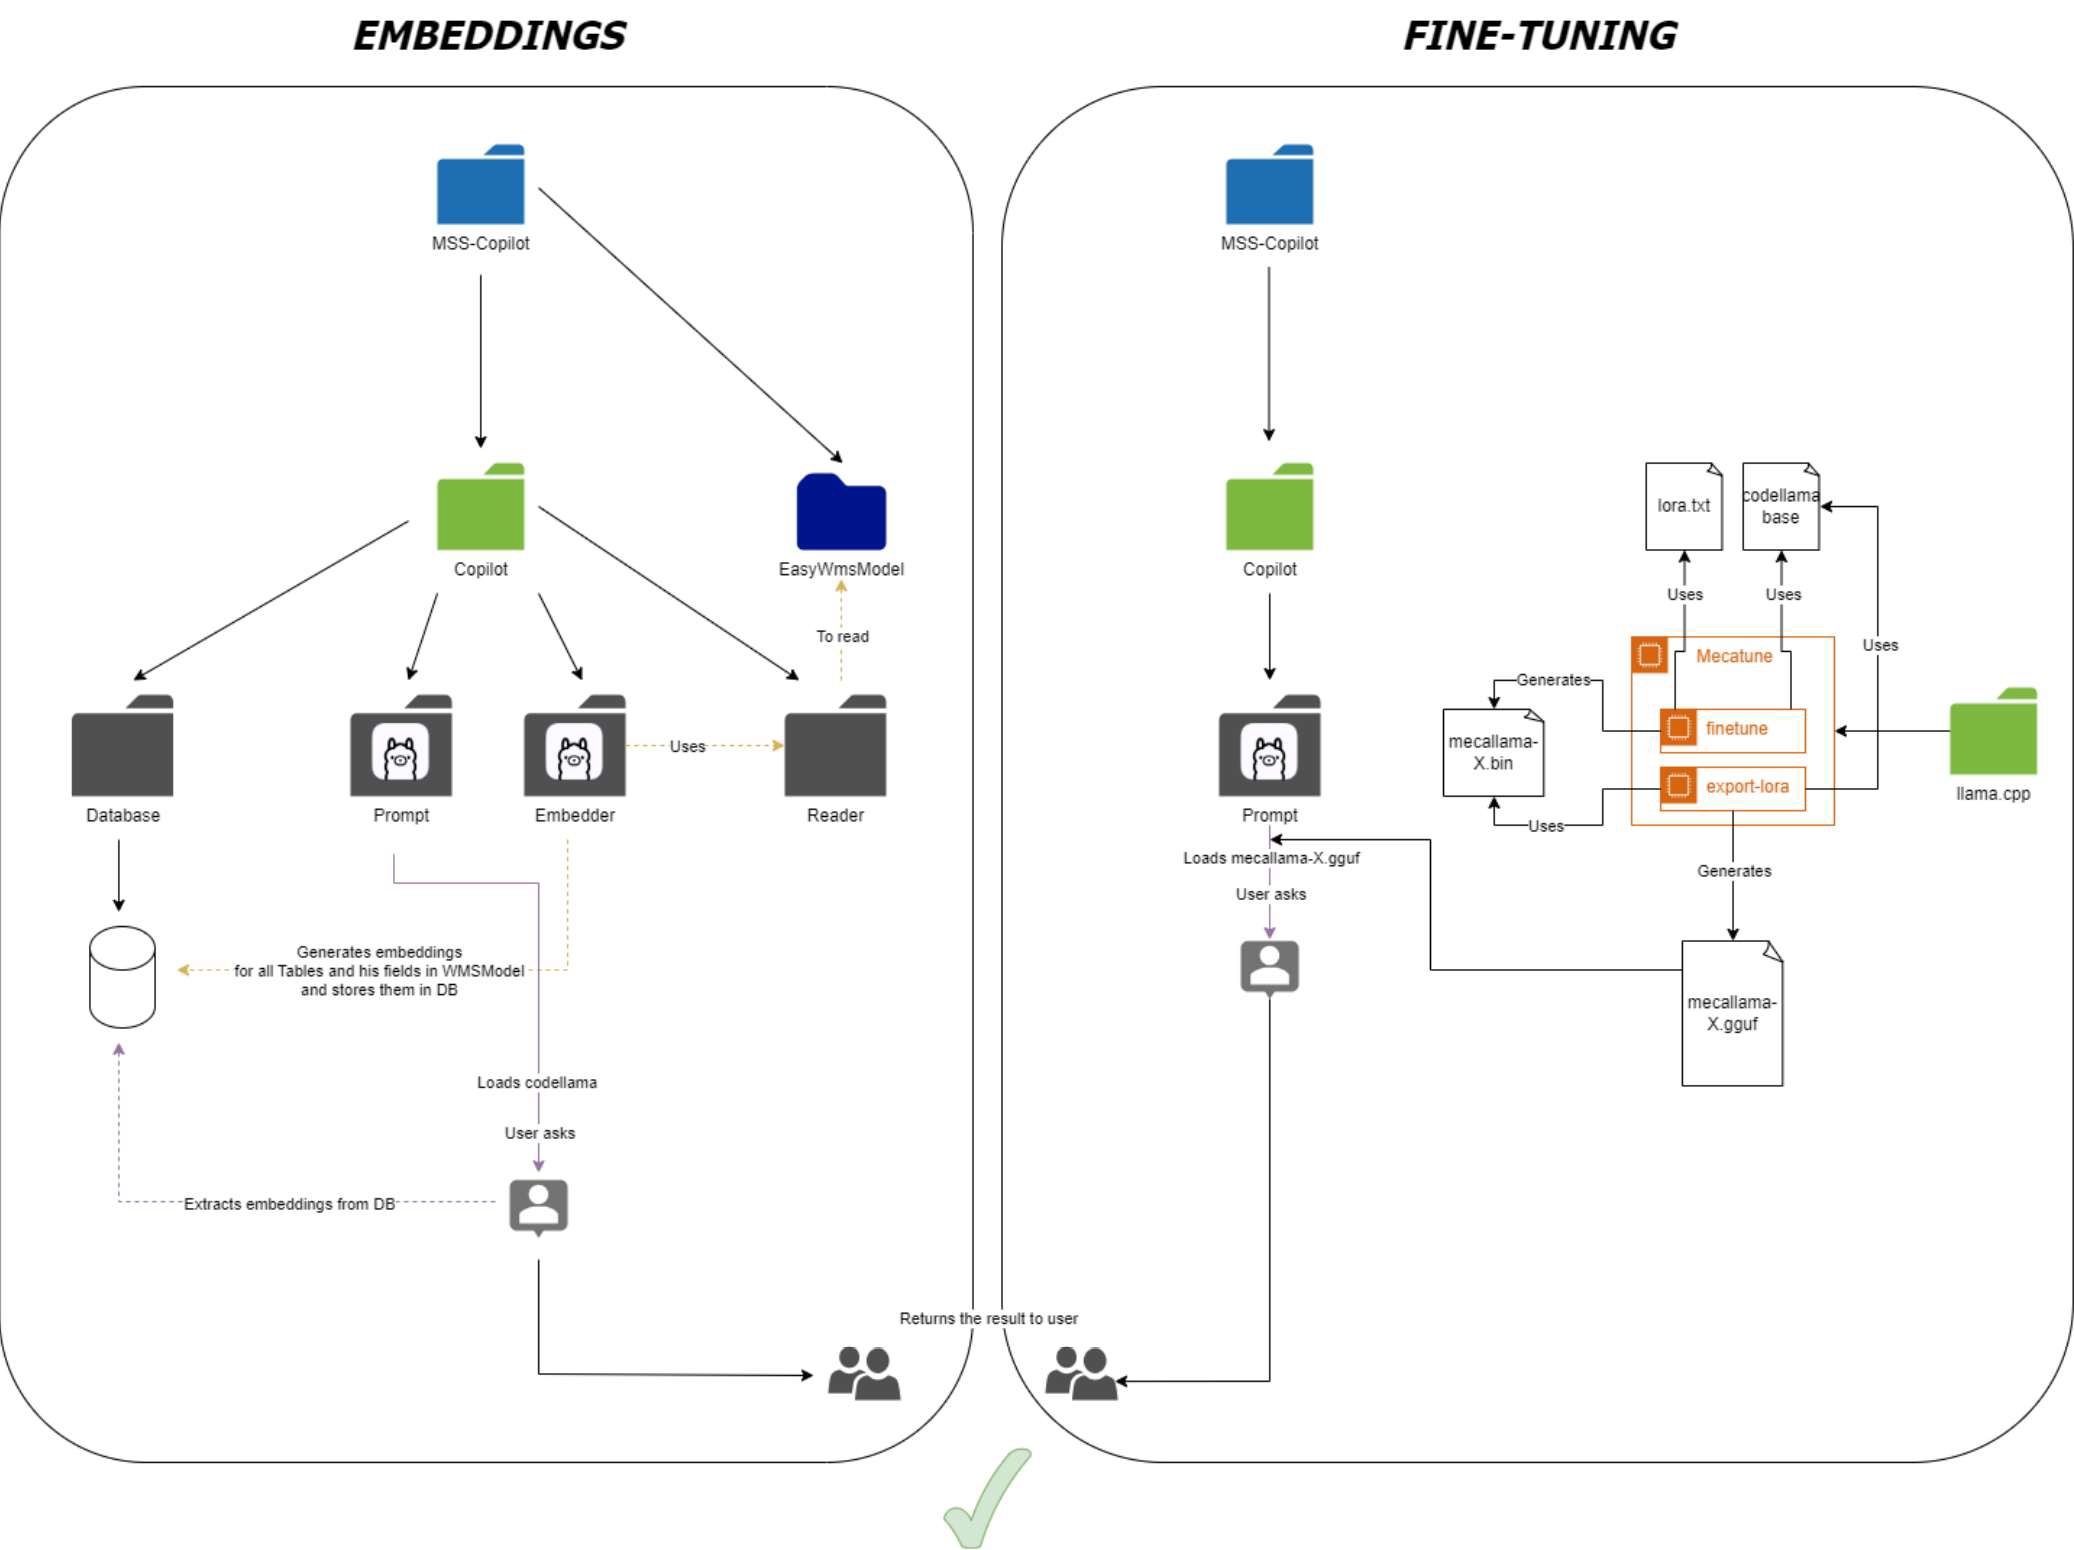
\includegraphics[width=1\textwidth]{Chapters/image.PNG}
    \label{fig:mi_imagen4}
\end{figure}

\newpage

\section{Relación de las tareas desarrolladas
con los conocimientos adquiridos
en los estudios universitarios}
Al reflexionar sobre mis estudios, identifico varias asignaturas y temas que han sido particularmente relevantes y valiosos para mi formación. Estos incluyen:
\begin{itemize}
    \item \bold{Sistemas Inteligentes e Inteligencia de Negocio:} Cursé Sistemas Inteligentes en el 2020-2021 e Inteligencia de Negocio el año posterior, así que no puedo ser muy específico en cuanto al temario dado pero creo que son dos asignaturas que aunque hayan pasado 2-3 años desde que las he cursado me han permitido realizar las prácticas con un contexto general sobre la inteligencia artificial, conceptos como el procesamiento del lenguaje natural, o el entendimiento de como funciona un \href{https://en.wikipedia.org/wiki/Large_language_model}{\bold{LLM}} por debajo, y conceptos como tokens, training data, sobreajuste, subajuste, etc..
    \item \bold{Bases de Datos y Sistemas de Información:}  Bases de datos ha sido una asignatura esencial ya no solo por el hecho de almacenar la información de los Embeddings sino que en el contexto del programa, que es un asistente de sentencias SQL, ha sido esencial para poder probar luego la IA y saber que las queries que me daba eran correctas o no, además de que en esta asignatura aprendí \href{https://www.postgresql.org/}{\bold{PostgreSQL}}. Destaco también la asignatura de Sistemas de Información porque en ella utilicé \href{https://www.sqlite.org/}{\bold{SQLite}}, y fue la primera toma de contacto que tuve entre backend y BDD.
    \item \bold{Metodología de la Programación y Tecnologías y Paradigmas de la Programación:} Del caso de Metodología de la Programación recalcar la importancia de haber aprendido polimorfismo, y de Paradigmas de la Programación los patrones de diseño, cabe recalcar que prácticamente todo el conocimiento backend de la carrera ha sido en \href{https://www.java.com/en/}{\bold{Java}}, y que \href{https://dotnet.microsoft.com/es-es/languages/csharp}{\bold{C\#}} se utiliza únicamente en las prácticas de Seguridad y muy muy superficialmente, pero con los conocimientos de estas asignaturas no ha sido nada complicado hacer una abstracción de todos estos conocimientos de programación y aplicarlos en \href{https://dotnet.microsoft.com/es-es/languages/csharp}{\bold{C\#}}, la adaptación fue bastante más amena de la que pensaba en un principio. 
    \item \bold{Programación Concurrente y Paralela:} Si bien he utilizado paralelización de tareas ha sido de una manera muy básica, ya que las librerías se encargaban de hacerlo todo más fácil, pero los conocimientos teóricos han sido útiles de igual manera, y recalcar sobre todo los contenidos aprendidos respecto a 
    \href{https://es.wikipedia.org/wiki/CUDA}{\bold{CUDA}}, el modelo \href{https://en.wikipedia.org/wiki/Large_language_model}{\bold{LLM}} se puede ejecutar tanto en CPU como GPU, y toda la problemática que implica programar utilizando 
    \href{https://es.wikipedia.org/wiki/CUDA}{\bold{CUDA}} se me hizo muy amena gracias a esta asignatura, sin ella se me hubiese hecho muy cuesta arriba este aspecto.
    \newpage
    \item \bold{Configuración y Evaluación de Sistemas:} Me ha parecido una asignatura fundamental y que he recordado muchas veces a la hora de realizar las prácticas, he tenido que hacer muchísimos benchmarks y pruebas de rendimiento frente a muchas casuísticas y hacer muchas gráficas que gracias a esta asignatura considero que he hecho correctamente. Me gustaría comentar que gracias al paradigma de esta asignatura me percaté que el programa daba unos tiempos de respuesta anormales y que eran debidos a dos factores principales, uno que la capacidad de cómputo era tal que el procesador llegaba al estrangulamiento térmico y capaba sus capacidades para no prenderse fuego, y que la discrepancia entre múltiples equipos del departamento se debía a que muchos de estos eran portátiles y su potencia se veía enormemente reducida cuando no estaban enchufados a la corriente independientemente de que se hubiese configurado Windows para que esto no pasase.
    \item \bold{Sistemas Distribuidos y Algoritmia:} Son dos asignaturas que en lo que es conocimientos no me han servido especialmente, quizás si Algoritmia de manera más subconsciente, pero son asignaturas en las que utilicé muchísimo \href{https://en.wikipedia.org/wiki/C_(programming_language)}{\bold{C}} y \href{https://en.wikipedia.org/wiki/C%2B%2B}{\bold{C++}}, lo cual me vino bien de cara a la parte de Fine-tuning.
    \item \bold{Sistemas Operativos:} Considero que es otra de las asignaturas fundamentales, ya que nos enseñan a manejarnos bien en un sistema basado en Linux, crear shell-scripts, y hacernos descubrir este aspecto de la informática y la importancia de la consola, que de no ser por esta asignatura, probablemente no tendría los conocimientos que tengo hoy en día. 
\end{itemize}